\chapter{Introduction}

\begin{figure}[htbp]
\centering
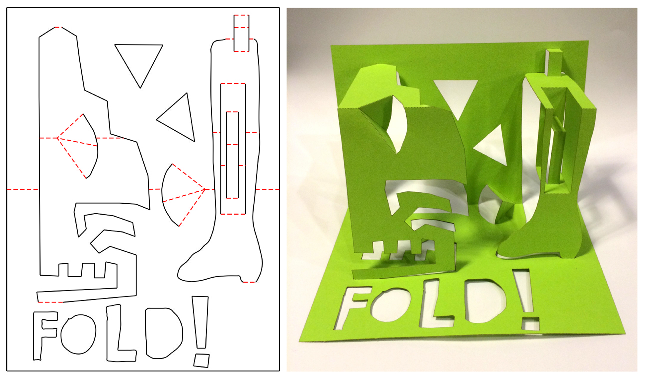
\includegraphics{figures/shared/01_Background/complexFoldlings.pdf}
\caption{A complex design created with our software.}
\end{figure}

\section{Background}\label{background}

\emph{This section is co-authored with Marissa Allen}

Kirigami is the art of papercraft originating from 17th century Japan
(\citet{temko1978magic}). Kirigami structures vary widely in form and
scale ---~from sub-microscopic creations to large sculptures
(\citet{grosso2015bending} to \citet{andrewscreating}). Kirigami can
represent a wide range of 2D and 3D constructions. For example, a design
can be a 2D lace-like pattern, or a large architectural structure; as
long as the paper design does not require glue or other attachments, it
is kirigami. Further constraints define subsets of kirigami --- such as
origami, which only allows folds\footnote{Purist origami adds further
  restrictions, including the requirement that the starting piece of
  paper be square (\citet{burczykul}).}. In particular, Foldlings is
concerned with 90-degree pop-up cards, which have the additional
constraint that orthogonal relationships exist between planes. We do not
use glue or other attachments in building pop-up cards; all designs are
cut from a single piece of paper, in the tradition of kirigami
(\citet{temko1978magic}). Thus, Foldlings creates orthogonal, kirigami
popup cards.

\begin{figure}[htbp]
\centering
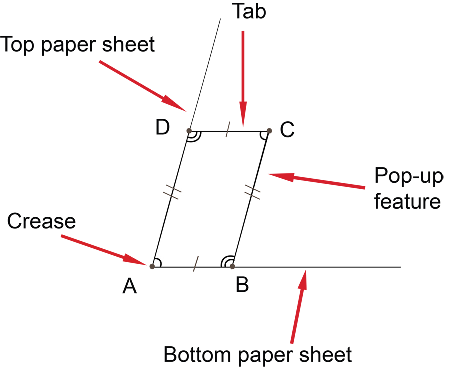
\includegraphics{figures/shared/01_Background/popup-diagram.pdf}
\caption{Cross-section of a popup card. Figure modified from
https://en.wikipedia.org/ wiki/File:Popup-diagram.svg.}
\end{figure}

Typically, users create popup cards manually. For example, a user might
sketch out shape on a card in pencil, and then measure with a rule to
determine locations to place folds. Or, they might fold the paper while
cutting, discovering correct fold positions experimentally. The second
method works well for simple designs, but becomes difficult with complex
and nested geometries\footnote{These are behaviors we observed by
  watching users create pop-up cards.}. Constructing popup cards
manually is difficult for several reasons:

\begin{enumerate}
\def\labelenumi{\arabic{enumi}.}
\itemsep1pt\parskip0pt\parsep0pt
\item
  \textbf{2D to 3D visualization is difficult}. Users have difficulty
  understanding how the card will fold based on a 2D design.
\item
  \textbf{Geometric constraints}. Pop-up cards present strict
  constraints, which are often unintuitive to novice designers.\\
\item
  \textbf{No "undo"}. Since pop-up card design is often a
  trial-and-error process, designers must sometimes make multiple
  versions of their card to test their design.
\item
  \textbf{Physical constraints}. In addition to the geometric
  constraints, the paper medium presents physical limitations on where
  edges can be placed.
\end{enumerate}

The 90-degree popup card presents a tightly-constrained problem, with
opportunities for both interface design and algorithm innovations. Our
work spans human-computer interaction, graph-based algorithms, and
algorithms for manipulating bezier paths and pop-up card structures. Our
culminating product is an iPad application.

We present a system for designing popup cards, whose audience is
deliberately broad. That is, our tool aims to make the design process
easier and more fun for users with all degrees of popup card design
experience.
